\documentclass[border=10pt]{standalone}

\usepackage{tikz}
\usepackage{tikzsymbols}
\usetikzlibrary{calc,patterns,shapes.geometric}

\def\centerarc[#1](#2)(#3:#4:#5){\draw[#1] ($(#2)+({#5*cos(#3)},{#5*sin(#3)})$) arc (#3:#4:#5);}

\begin{document}
	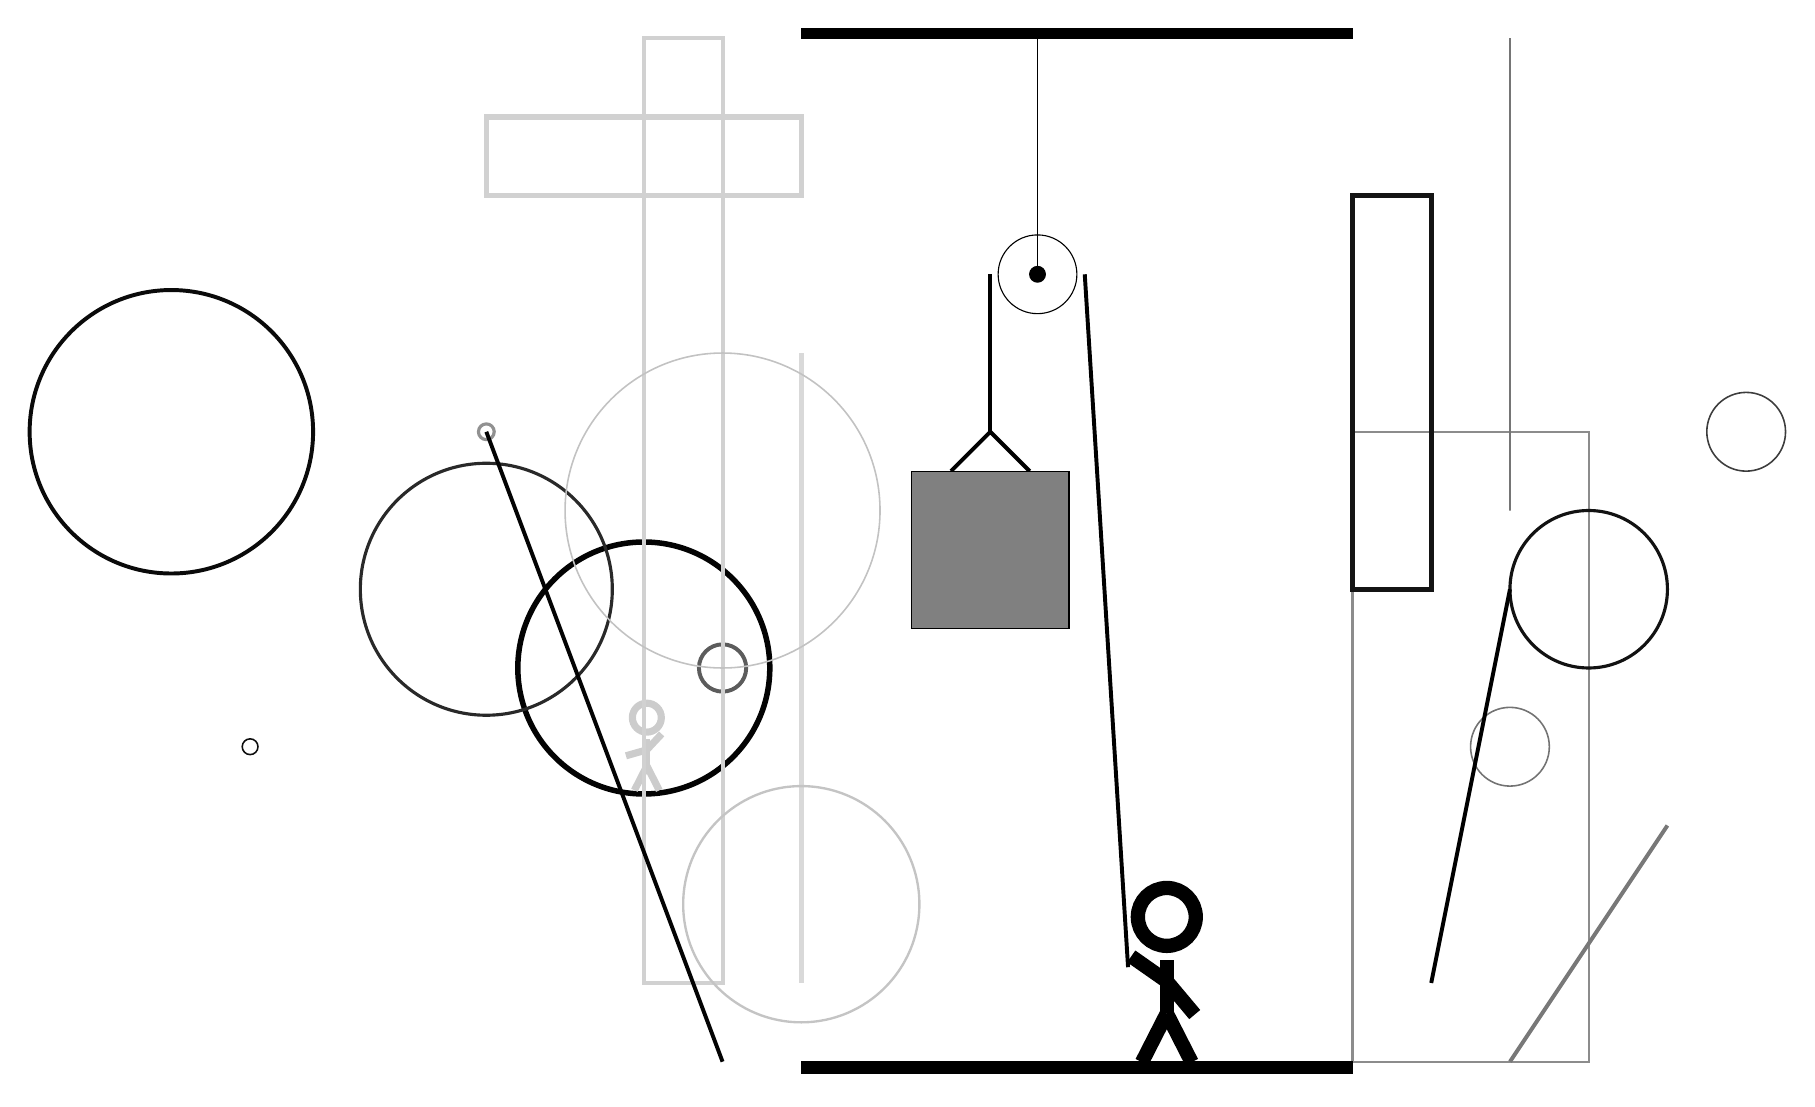
\begin{tikzpicture}
		%%%%% START %%%%%
		
		\draw[fill=black] (-2, 10) rectangle (5, 10.125);
		
		\draw[line width=0.3mm, color=black!45] (5, -3) rectangle (8, 5);
		
		\draw [line width=0.4mm, color=black!43](-6, 5) circle (0.1);
		\draw [line width=0.7mm, color=black!99](-4, 2) circle (1.6);
		\node[line width=0.5mm, color=black!20] at (-4, 1) {\Strichmaxerl[5][16][47]};
		\draw[line width=0.6mm, color=black!15] (-2, 6) rectangle (-2, -2);
		\draw [line width=0.5mm, color=black!96](-10, 5) circle (1.8);
		\draw [line width=0.4mm, color=black!84](-6, 3) circle (1.6);
		\draw [line width=0.5mm, color=black!64](-3, 2) circle (0.3);
		\draw[line width=0.5mm, color=black!18] (-4, 10) rectangle (-3, -2);
		
		\draw [line width=0.2mm, color=black!55](7, 1) circle (0.5);
		\draw [line width=0.4mm, color=black!93](8, 3) circle (1.0);
		
		\draw[line width=0.7mm, color=black!18] (-2, 9) rectangle (-6, 8);
		\draw[line width=0.5mm, color=black!100](7, 3) -- (6, -2);
		
		\draw[line width=0.5mm, color=black!99](-6, 5) -- (-3, -3);
		\draw [line width=0.3mm, color=black!23](-2, -1) circle (1.5);
		\draw[line width=0.2mm, color=black!54] (7, 4) rectangle (7, 10);
		
		\draw[line width=0.5mm, color=black!21](6, 7) -- (6, 3);
		\draw[line width=0.6mm, color=black!92] (6, 8) rectangle (5, 3);
		\draw [line width=0.2mm, color=black!24](-3, 4) circle (2.0);
		
		\draw [line width=0.2mm, color=black!95](-9, 1) circle (0.1);
		\draw [line width=0.2mm, color=black!76](10, 5) circle (0.5);
		\draw[line width=0.5mm, color=black!53](9, 0) -- (7, -3);
		
		\draw (1, 7) circle (0.5);
		\draw[fill=black] (1, 7) circle (0.1);
		\draw (1, 10) -- (1, 7);
		
		\draw[line width=0.5mm] (-0.1, 4.5) -- (0.4, 5.0) -- (0.9, 4.5);
		\draw[fill=black!50] (-0.6, 4.5) rectangle (1.4, 2.5);
		
		\draw[line width=0.5mm] (0.4, 7) -- (0.4, 5.0);
		\centerarc[line width=0.5mm](1, 7)(0:180:0.6);
		\draw[line width=0.5mm](1.6, 7) -- (2.15, -1.8);
		
		\node at (2.6, -1.9) {\Strichmaxerl[10][-35][-50]};
		
		\draw[fill=black] (-2, -3) rectangle (5, -3.15);
		
		%%%%% END %%%%%
	\end{tikzpicture}
\end{document}